\section{Anomaly Detection Methods}
\label{sec:methods}

----Introduce section

As part of the data reduction procedure, a moving average was applied to data in both the time domain and the frequency domain. A moving average essentially applies a low-pass filter to the data.

For the time domain, this was mainly applied in order to ensure more accurate reconstructions when using techniques such as K-mean Clustering Reconstruction (see \S~\ref{subsec:kmeans}) and LSTM Recurrent Neural Networks (see \S~\ref{subsec:LSTM}).

For the frequency domain, the moving average was applied to the frequency domain, after the Fourier transform has already been applied to the unaltered time series data. This ensures that all of the higher frequencies were not lost.

The method of taking a moving average is implemented using the convolution of the data with a kernel, $k$. If a moving average with width $w$ is required, the kernel is defined as,

\begin{equation}
    k = \left[ \dfrac{1}{w}~\dfrac{1}{w}~\dfrac{1}{w}...\dfrac{1}{w}  \right]~,
    \label{eq:conv_kernel}
\end{equation}

where the array is of length $w$. This is then convolved with the data set, which has the effect of `smoothing' the data.

\begin{figure}[t]
    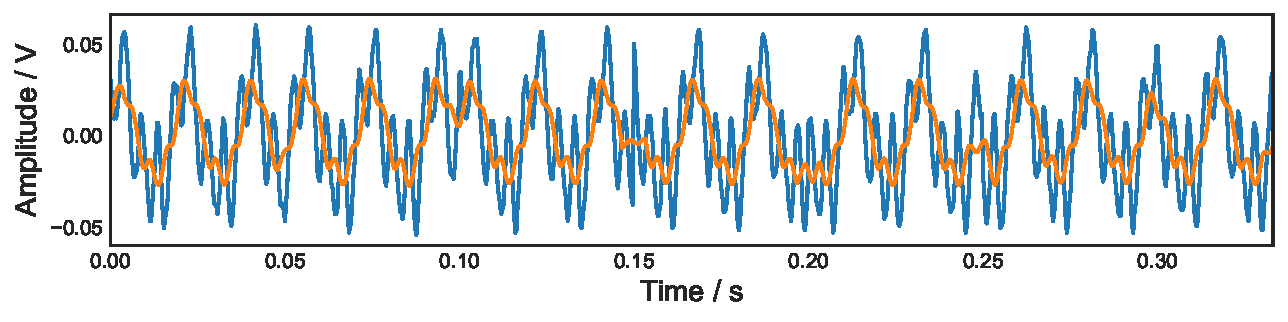
\includegraphics[width=1.0\textwidth]{fig/moving_average.pdf}
    \caption[Time Domain]{Moving average applied to data in the time domain. The original data (shown in blue) represents the amplitude of the signal as a function of time. The orange curve shows the moving average of this data.}
    \label{fig:moving_av}
\end{figure}

\begin{figure}[t]
    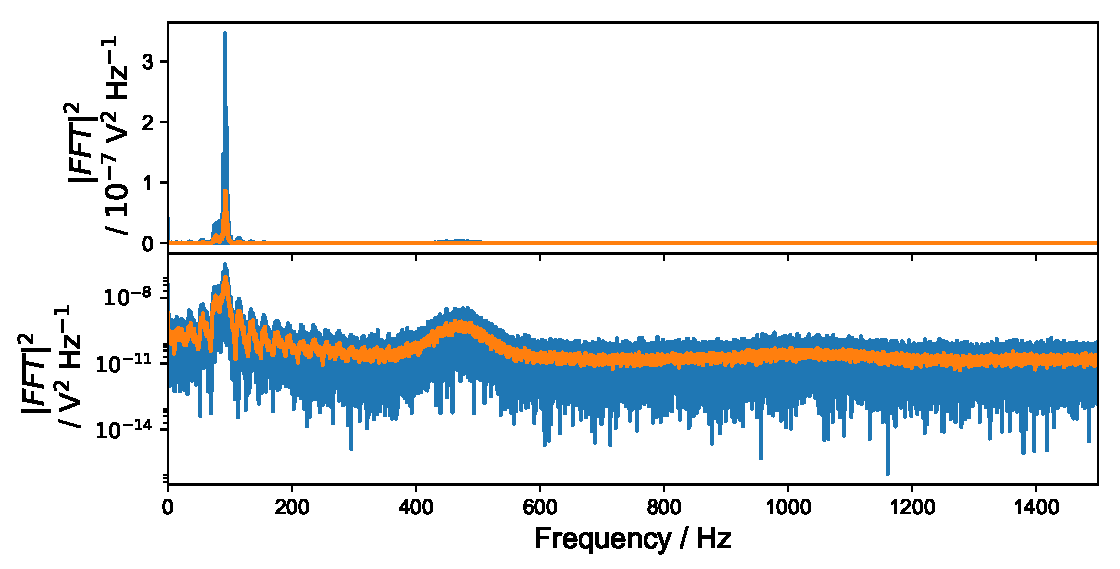
\includegraphics[width=1.0\textwidth]{fig/freq_moving_average.pdf}
    \caption[Moving Average in Fourier Domain]{Moving average applied to data in the Fourier domain, shown in both linear and logarithmic axes. The blue lines show the original amplitudes as a function of frequency. The orange lines show the moving averages.}
    \label{fig:freq_moving_av}
\end{figure}

Figures.~\ref{fig:moving_av} and ~\ref{fig:freq_moving_av} show examples of applying a moving average to data in the time domain and frequency domain, respectively. 


----Moving average for dealing with issues with the resloution for the raw data in the y axis

\subsection{Statistical Approach}

The most simple methods for detecting changes from `normal' motor behaviour can either use simple value thresholds, or static mean and standard deviation calculates to determine when data experiences a significant deviation from usual patterns. 

Such basic approaches are not easily adapted for use in time series data. This is because:

\begin{enumerate}
    \item These methods are not easily applied to changing data values.
    \item They cannot scale easily to large time series.
    \item An unacceptable quantity of false anomalies can be detected.
    \item They rely on the assumption of a normal distribution of data points, which is not always the case for time series data.
\end{enumerate}

Nevertheless, these approaches can provide immediate indications of the most obvious anomalies. 

In order to ensure that the data the statistical tests were applied to followed a Gaussian distribution, a moving average was first taken.

\begin{figure}[t]
    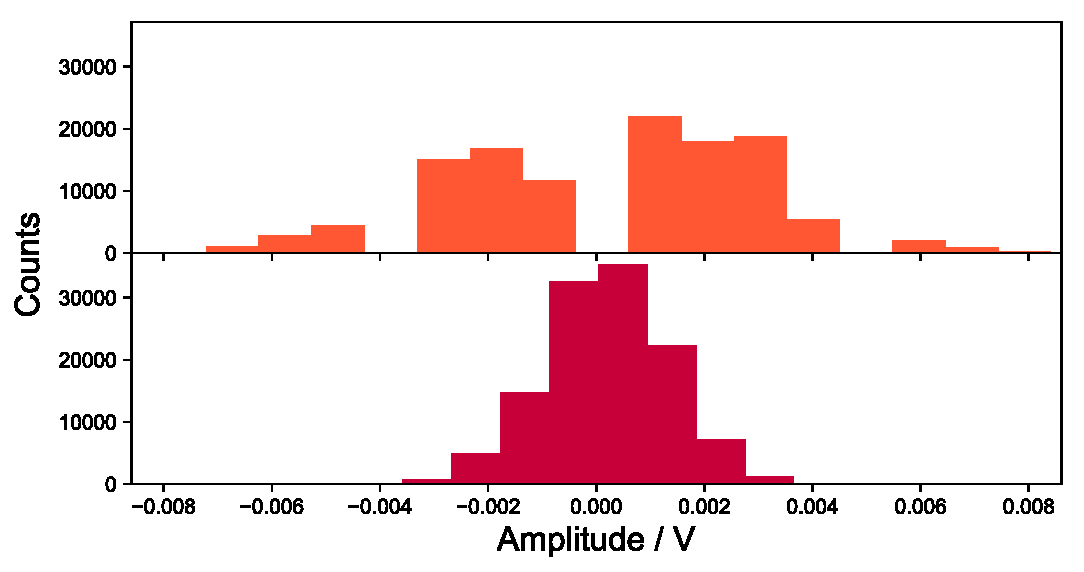
\includegraphics[width=1.0\textwidth]{fig/moving_av_hist.pdf}
    \caption[Moving Average Histogram]{Histograms for the raw data (top) and when a moving average with a window size of $w=20$ is applied (bottom).}
    \label{fig:move_av_hist}
\end{figure}

Figure.~\ref{fig:move_av_hist} shows how the distribution for the moving-averaged data has a Gaussian distribution, whereas the raw data does not.

It was therefore necessary to apply a moving average to the raw data before any statistical tests were performed.

\subsubsection{Histogram Test}

\begin{figure}[t]
    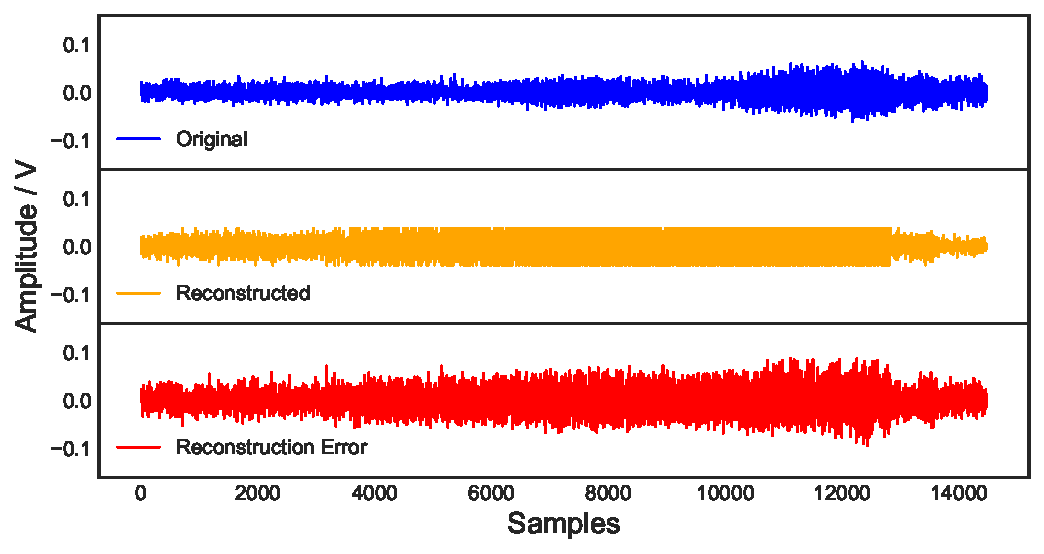
\includegraphics[width=1.0\textwidth]{fig/histogram.pdf}
    \caption[Histogram]{Histogram method}
    \label{fig:histogram}
\end{figure}

The histogram test first assumes that the recorded data is normally distributed, so that the probability $p$ of a value $x$ is,

\begin{equation}
    p(x) = \dfrac{1}{\sigma \sqrt{2\pi}}\exp(\dfrac{-{(x-\mu)}^2}{2\sigma^2})~,
\end{equation}

where $\mu$ and $\sigma$ are the mean and standard deviation of the sample respectively.

The method begins by separating the a `training' time series sample into equal bins. This training sample serves as a set of example data that represents the expected behaviour. The median value of each of these bins is then calculated.

A reconstruction of a time series is then carried out. For each value in the time series, the difference between the defined medians, and the value is calculated. The smallest difference is then chosen to represent the reconstruction of the time series.

Figure.~\ref{fig:histogram} shows an example of the histogram method for an arbitrary time series. The reconstruction error represents the difference between the original time series and the reconstructed time series. The training data was taken from a motor operating at the same voltage as the test data, under normal baseline conditions.

\subsubsection{Grubbs' Test}
One of the most commonly used statistical threshold tests for outliers is the two-sided Grubbs' Test \cite{CIS-320511}.

For the two-sided Grubbs' test, this involves defining a Grubbs' test statistic as,

\begin{equation}
    G = \dfrac{\underset{i=1,2,...,N}{\max}|\mathcal{X}_i-\bar{\mathcal{X}}|}{\sigma}~,
    \label{eq:grubbs}
\end{equation}

where $\mathcal{X}$ denotes a set of data of length $N$, and $\bar{\mathcal{X}}$ and $\sigma$ are the mean and standard deviation of this data set, respectively. $G$ is equivalent to the largest deviation from the mean in units of standard deviations.  

The hypothesis of no outliers being present is rejected if,

\begin{equation}
    G > \dfrac{N-1}{\sqrt{N}} \sqrt{\dfrac{(t_{\alpha/(2N), N-2})^2}{N-2+(t_{\alpha/(2N), N-2})^2}} ~,
    \label{grubbs_condition}
\end{equation}

where $t_{\alpha/(2N), N-2}$ denotes the $t$-distribution with a significant level of $\alpha/(2N)$ and $(N-2)$ degrees of freedom. 

The Grubbs' test is useful in identifying if an outlier exists in the data set, however it is very limited. It only identifies if the data is anomalous, and does not indicate how many anomalies there are or indicate where in time the anomalies are.

Nevertheless, it can be used as a very quick indication of whether results are anomalous in amplitude over time. If it indicates outliers are present, more rigorous statistical tests can be used to determined where and when outlier occurred. 

\subsubsection{Standard Deviation Test}
Assuming that a data set is normally distributed, a simple threshold test on the residuals from the mean can be used to detect outliers. 
Although a deviation of more than $3\sigma$ can in some cases be considered to be anomalous, there is still a $0.3\%$ chance of a data point following the normal distribution to fall more than $3\sigma$ from the mean. In some cases, the data sets analysed in this report can exceed $100,000$ entries. Using a $3\sigma$ threshold test in this case would lead to $300$ false positives. Alternatively, with a sampling rate of $3000$ Hz, this would equate to $9$ incorrect outlier alerts every second. 

Instead, $5\sigma$ was used as the threshold for the residuals. The likelihood of a normal data point deviating from the mean by more than $5\sigma$ is $3 \times 10^{-7}$, giving a much lower false positive detection rate of one every $\sim 18$ minutes. 

Therefore for the purpose of this report, a data point deviating by more than $5\sigma$ from the mean is considered to be an anomaly. 

This method can be used to find multiple anomalies within a data set, with their respective positions in time.

\subsubsection{Deviation From Moving Average}
This is a similar method to the standard deviation test, but instead of calculating the mean and standard deviation of the entire sample, a moving mean and standard deviation are taken. A window size of 50 for the moving average was used.
If a data point deviates from the moving average by 4 moving standard deviations or more, then it is considered to be an outlier. This method is better for detecting just the anomalies at shorter time scales, whereas the Standard Deviation Test detects both short scale and more gradual amplitude changes. 

Unlike the previous two tests, this is applied to the raw data, as the test itself involves smoothing the data and comparing this to the raw data.


\subsection{Fourier Analysis}

\begin{figure}[t]
    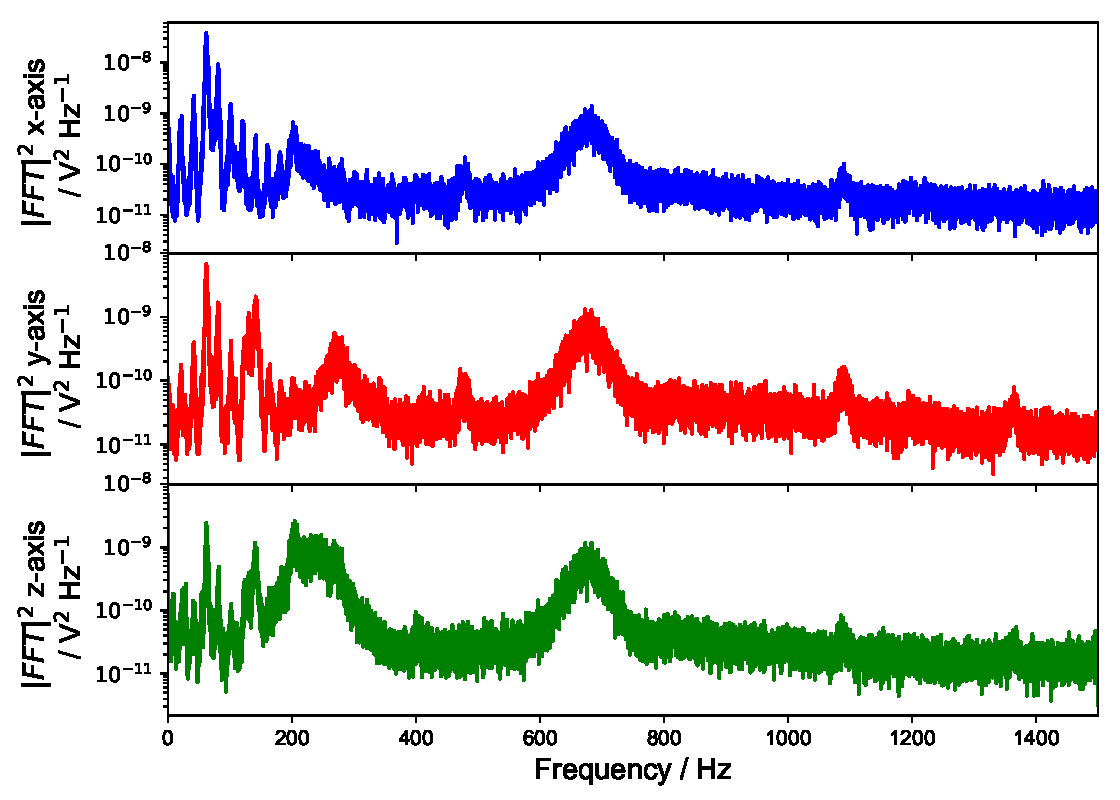
\includegraphics[width=1.0\textwidth]{fig/freq_theory.pdf}
    \caption[Fourier Spectrum of 12 V motor in $xys$ axes]{Amplitudes as a function of frequency for the 12 V motor in all 3 axes. }
    \label{fig:frequencies}
\end{figure}

Fourier transforms of time series data are used to provide a mapping between the time domain and the frequency domain, finding the amplitude of the constituent frequencies \cite{hsu_1984}. Another term for this frequency domain representation is the spectrum of the signal. 

This transformation was implemented using a Fast Fourier Transform (henceforth FFT), in order to perform a discrete fourier transform (DFT). If time series data consists of a set of data of length $N$, $\{ x_0, x_1,...,x_{N-1} \}$, the DFT is defined as \cite{hsu_1984},

\begin{equation}
    y_k = \sum_{m=0}^{N-1} x_m \cdot e^{-2\pi ikm/N} \quad (k = 0,1,...,N-1)~,
    \label{eq:DFT}
\end{equation}

where $y_k$ is the amplitude for a given $k$. $k$ is related to frequency, and the frequency $f$ can be obtained using the equation,

\begin{equation}
    f = \dfrac{k}{N} \times S~,
    \label{eq:freq_from_k}
\end{equation}

where $S$ is the sampling rate with which the data was collected ($S=3000$ Hz for this work). Therefore Eq. \eqref{eq:DFT} returns values of $y_k$, for $k = 0,1,...,N-1$, making $N$ values in total, that correspond to amplitudes for equally spaced frequencies between $0$ and $3000$ Hz. However, due to the Nyquist-Shannon Sampling Theorem (see \S\ref{subsec:anomaly_detection}), only the first half of these frequencies can be properly resolved, and so the second half of the $y_k$ values are discarded.

When representing the spectrum, the power spectral density (PSD) was used, which is found by multiplying the complex amplitude obtained from the $FFT$ by its complex conjugate, giving $|FFT|^2$. This is useful as it is proportional to the power output per unit frequency, and in addition makes peaks more visually prominent in the spectrum. The $|FFT|^2$ was then normalised by dividing by $N$, the length of the data, to ensure the amplitudes of peaks in Fourier space do not depend on the length of data used to generate them (so that a spectrum taken from 2 seconds of data will have the same amplitudes as one taken from 2 minutes of data).

Figure~\ref{fig:frequencies} shows the power spectral density returned using this method. A logarithmic axis is used to make the less prominent peaks visible.

\subsubsection{Gaussian fitting in frequency space}

In addition to visual inspection of the spectra, a more quantitative approach was attempted. This was achieved by fitting a Gaussian curve to the most prominent peak in the spectrum. This was done by varying the parameters of the Gaussian and using a least-squares regression algorithm to minimise the residuals between the data and the Gaussian curve. A Lorentzian curve was also attempted, but the Gaussian generally gave a smaller sum of residuals and so is the method used. 

A Gaussian peak is defined by,

\begin{equation}
   \mathcal{G}(f) = A e^{-(f-\mu)^2/2\sigma^2}~,
    \label{eq:gaussian}
\end{equation}

where $A$ is the amplitude of the Gaussian, equal to the maximum amplitude of the peak; $\sigma$ describes the width of the peak and is related to the full-width at half-maximum (FWHM) by $FHWM = 2\sigma \sqrt{2ln2}$, and $\mu$ is the frequency of the centre of the peak. The total area under the peak is given by $\sqrt{2\pi}\sigma A$.

Time series data from a "healthy" motor (one in which no possible faults have been purposefully imposed) were subdivided into segments and spectra obtained in all three motor axes. These were used to generate a set of Gaussians for the most prominent peak in each, each described by the three parameters $A$, $\sigma$ and $\mu$, defined above.

Initially, baseline data was split into three second segments and a Fourier spectrum was obtained for each segment. A Gaussian curve was fitted to the most prominent peak in each spectrum. This was used to create a database of values for $A$, $\sigma$ and $\mu$ from each segment. From this, a mean and standard deviation (error) was obtained for $A$, $\sigma$ and $\mu$. 

This process was then repeated for data that was recorded when trying to induce failures, in order to again determine values for $A$, $\sigma$ and $\mu$ with their respective errors. If any of $A$, $\sigma$ or $\mu$ do not agree within their errors with the values obtained from the "healthy" baseline data, then there is an indication that the frequency response of the motor is changing. This technique can be very useful in autonomously tracking the frequency response of a motor. As many failure modes can manifest themselves as gradual changes in the frequency of the motor, this technique can be useful for detecting signs of failure that the statistical tests applied to amplitudes in the time domain fail to identify. 
 
\subsubsection{Harmonic Frequencies}


\subsection{Least Squares Anomaly Detection}
Included amongst our anomaly detection methods is a squared-loss objective function which is quick to detect anomalous data given a set of training and testing datasets. Due to the rudimentary nature of the function and the very simple analytical solution it has a speed advantage over other methods, as well as presenting a static anomaly score across the train and test data to visualise the magnitude of the anomalous data points. It can also be used to evaluate the difference between sub-sequences and therefore isn't invalidated when the dataset contains structural dependence.


\begin{itemize}
\item Moving average
\item Median filters
\item Comparison with SVM \& anomaly scoring
\end{itemize}

\begin{figure}[t]
    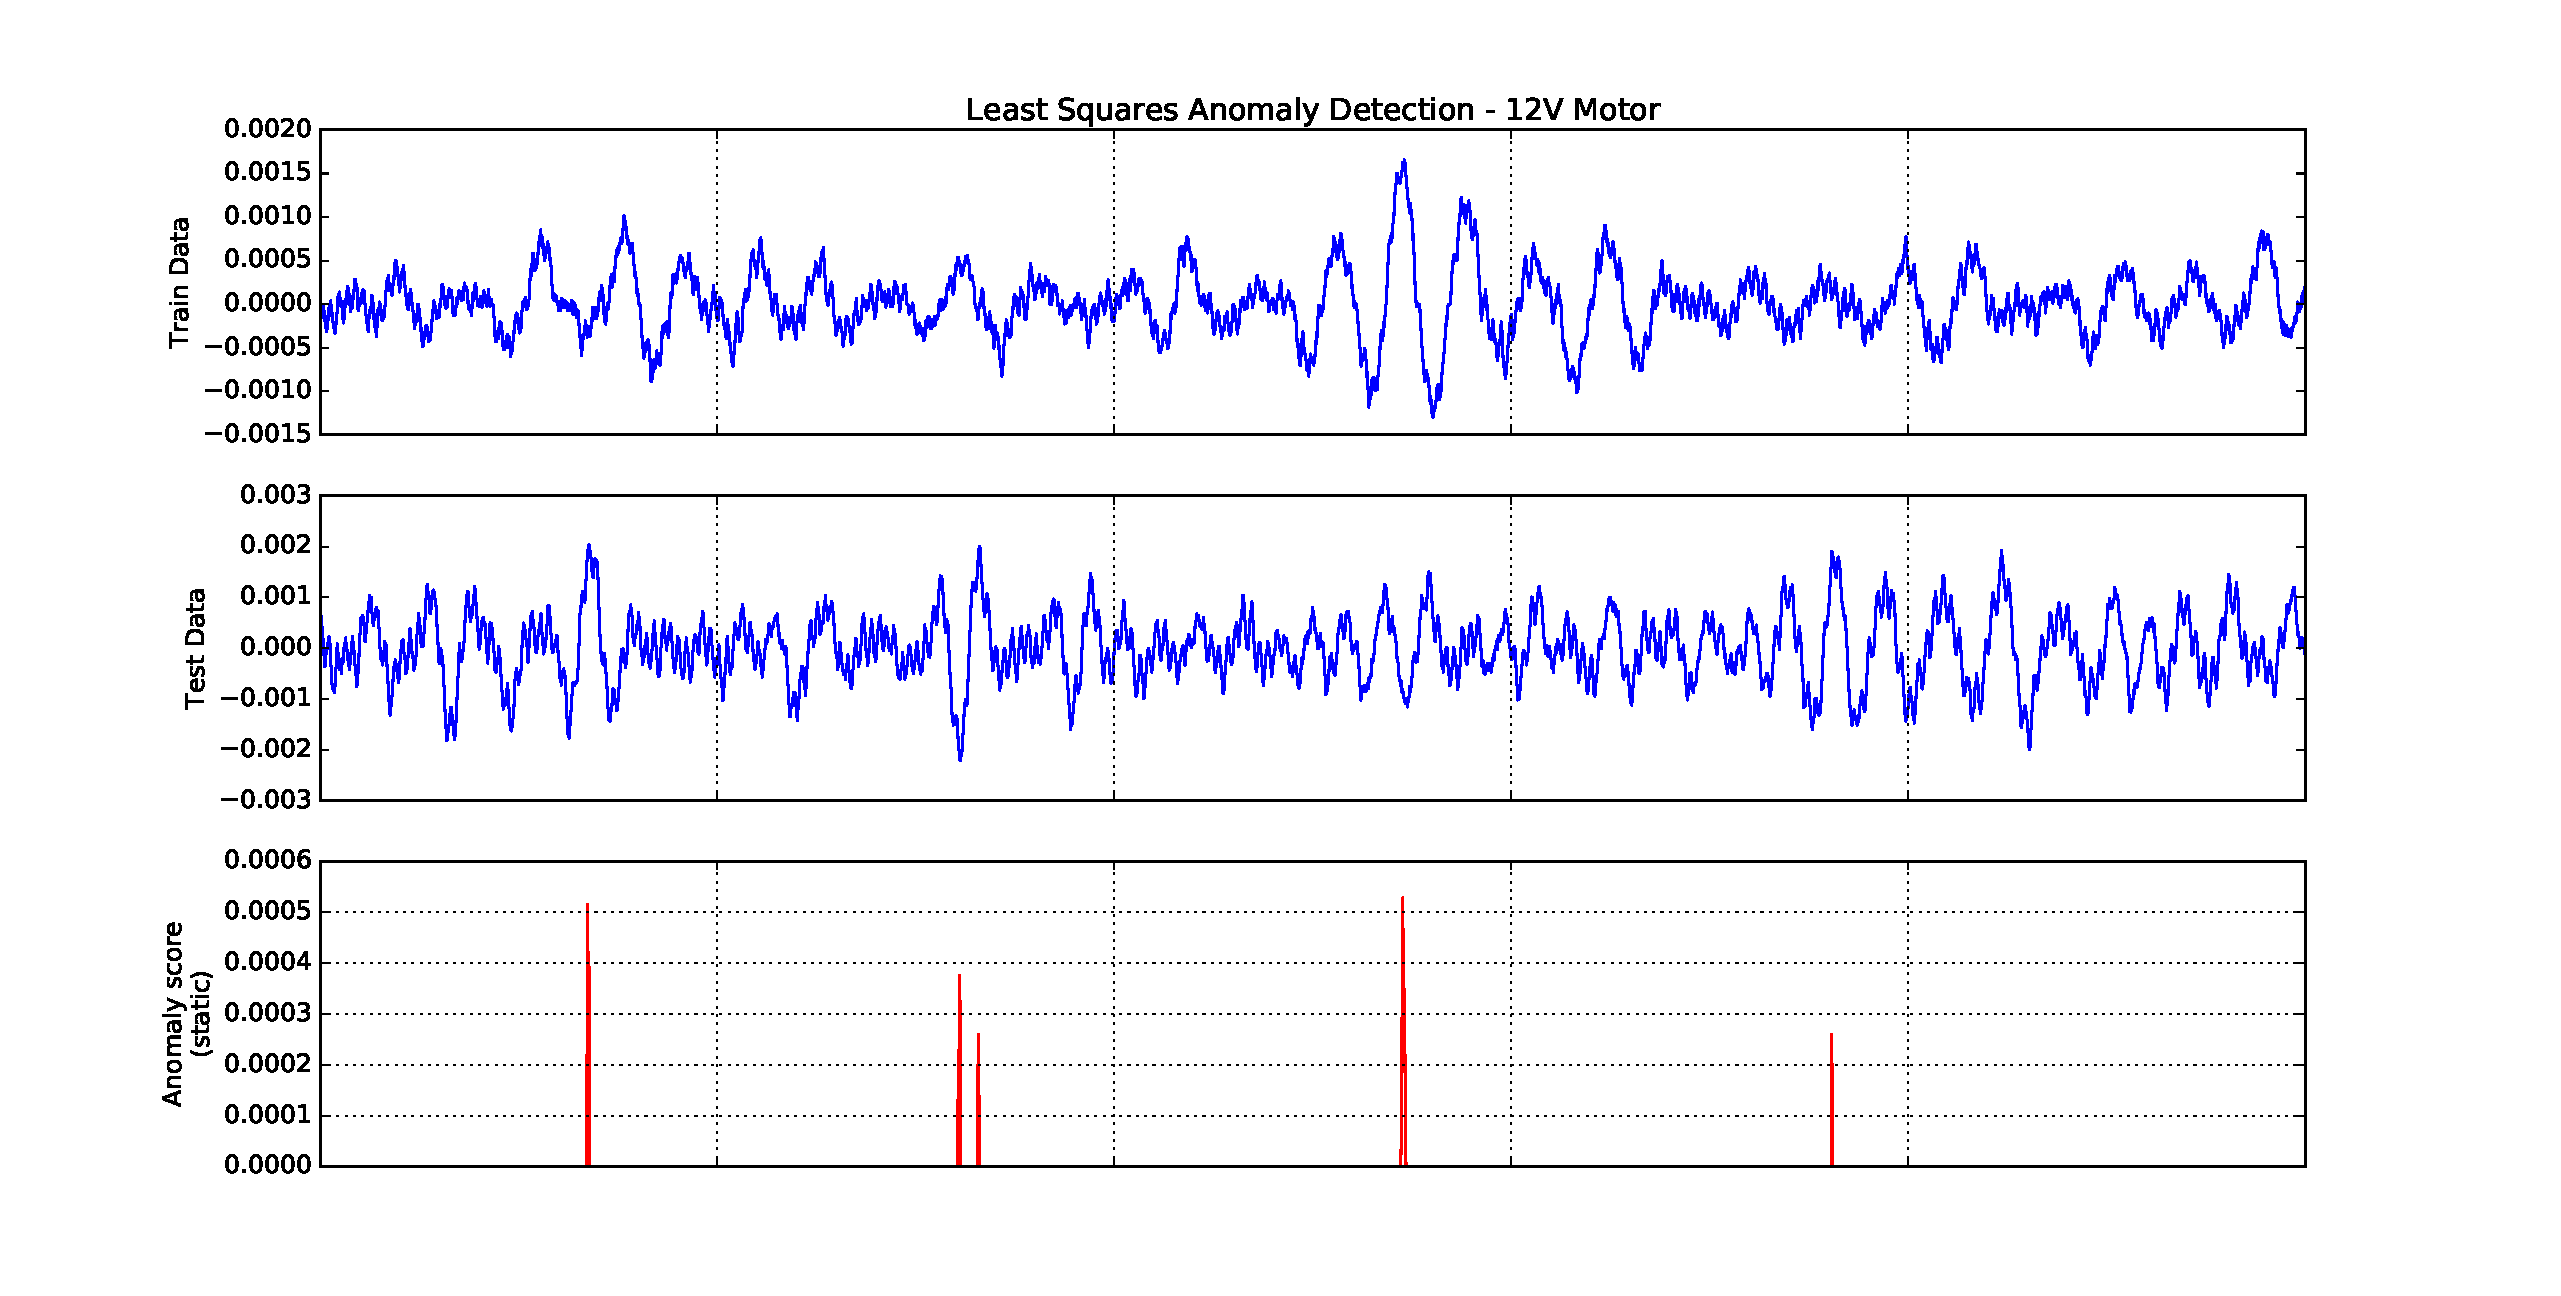
\includegraphics[width=1.0\textwidth]{lsanomaly.pdf}
    \caption[Least Squares Anomaly Score]{Spruced up plot here.}
    \label{fig:lsanomaly}
\end{figure}

\subsection{K-Means Clustering}
\label{subsec:kmeans}

Cluster analysis involves combining data points into groups, or clusters, in such a way that the points in each cluster are more similar to each other than other points outside of the cluster. Any data points that do not belong to a cluster are defined as outliers. 

Figure~\ref{fig:anomalies} in \S \ref{sec:introduction} shows an example of clusters in 2 dimensions. 

K-means clustering is one of the most highly used cluster analysis methods, due to it being much less computationally intensive in comparison to other approaches \cite{Kanungo:2002:EKC:628329.628801}.

The process involves partitioning a set of n-dimensional data points, of length $N$ ($\{\underline{x}_j\}$ for $j=1,2,...,N$) into a group of $k$ clusters, where $k$ has to be specified by the user. K-means aims to find the centroids $\underline{\mu}_i$ (with $i=1...k$), of the clusters that minimise the Euclidean distance from all data points to their respective clusters, $d(\underline{x}, \underline{\mu}_i) = ||\underline{x}-\underline{\mu}_i||^2$. More formally, K-means clustering finds the centroids of $k$ clusters in order to minimise the expression \cite{596afe3f2b5a4ff3b8f4f9793ad2f4ee},

\begin{equation}
    arg\,min_k \sum_{i=1}^{k} \sum_{\underline{x} \epsilon c_i} ||\underline{x}-\underline{\mu}_i||^2 ~,
    \label{eq:K-means}
\end{equation}

where $c_i$ are the points closest to the cluster $i$.

The general process is described as follows:
\begin{enumerate}
    \item Initialise the centre of the $k$ clusters randomly in Euclidean n-space.
    \item Attribute each data point to the closest cluster centre for that data point. 
    \item Assign a new position for the cluster centre, now given by the barycentre of the data points belonging to the cluster.
    \item Repeat steps 2 and 3 until convergence to a solution is achieved.
\end{enumerate}

Figure~\ref{fig:anomalies} in \S \ref{sec:introduction} shows an example of clusters in 2 dimensions. 

In order to apply K-means clustering to time series data, the n-dimensional space in which the clusters are defined first had to be defined. 

The entire signal waveform was split into segments in time, with each segment consisting of 24 data points. These segments will then be defined by a set of features, which will form the n-dimensional space. For example, the features could be the mean value and standard deviation of each segment, in which case a 2-dimensional space would be considered. Instead, in order to ensure no information is lost, each element in the 24-element segment is taken to be a separate dimension. Therefore a segment is completely specified by a single point in 24-dimensional space \cite{lin_vlachos_keogh_gunopulos_2004}.

All of the segments that make up the total waveform can then be plotted in this 24-dimensional space. Segments with similar features will cluster together. If $k$ clusters are defined, then the centroids of each cluster can be found to give $k$ coordinates in the 24-dimensional space, one for each centroid. Figure~\ref{fig:kmeans_training} shows ten random segments, taken from the original waveform, also known as the "training data".

The centroids, being points in the defined 24-dimensional space, are themselves waveform segments. These waveform segments will be referred to as synthetic segments, as they were generated from the input data but aren't themselves a part of the original data. 

\begin{figure}[t]
    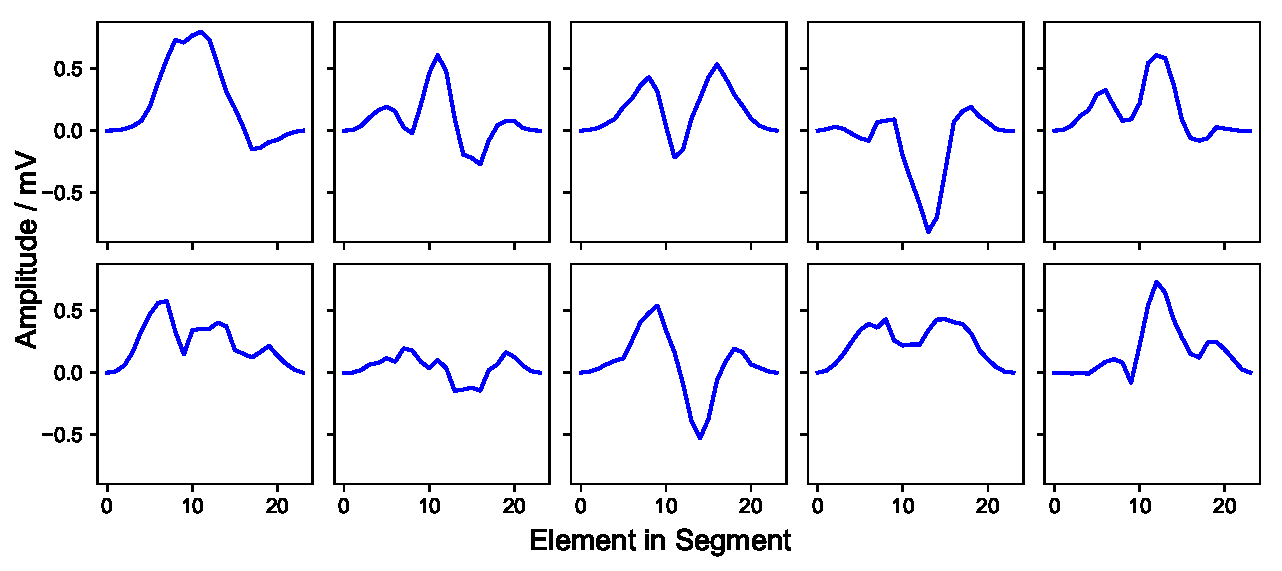
\includegraphics[width=1.0\textwidth]{fig/kmeans_training.pdf}
    \caption[K-means training segments]{A random selection of training segments, with windowing applied.}
    \label{fig:kmeans_training}
\end{figure}

\begin{figure}[t]
    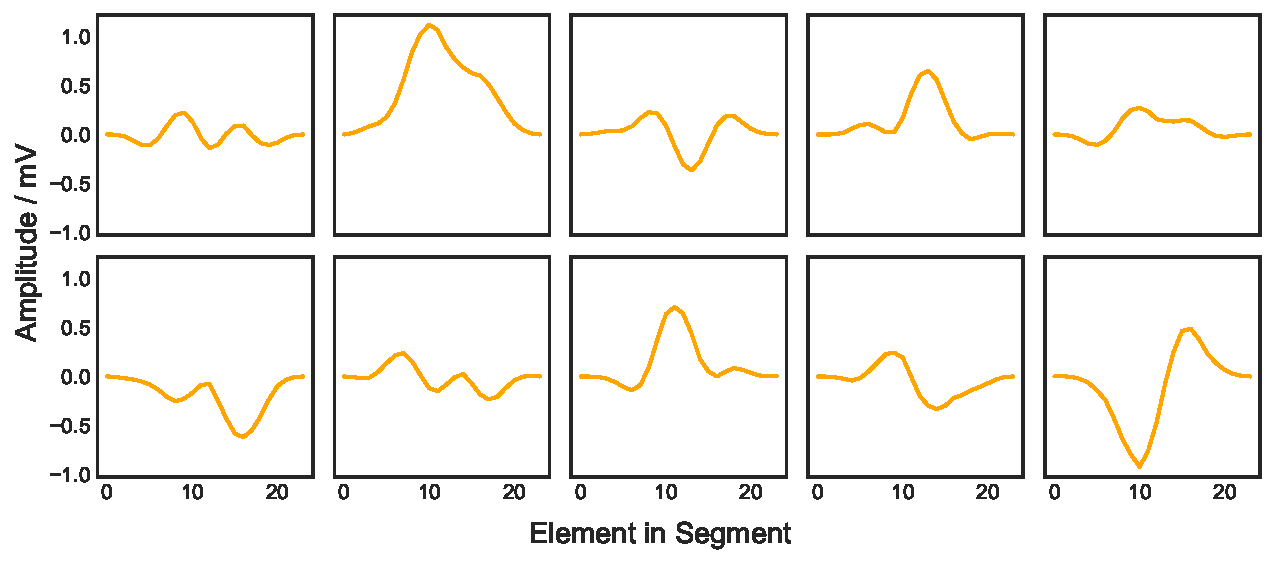
\includegraphics[width=1.0\textwidth]{fig/kmeans_synthetic.pdf}
    \caption[K-means synthetic segments]{A random selection of synthetic segments, generated from the centroids of clusters.}
    \label{fig:kmeans_synthetic}
\end{figure}

This creates a "library" of $k$ synthetic waveforms, which can be stitched together in order to recreate the original total signal. Figure~\ref{fig:kmeans_synthetic} shows a random selection of ten of these synthetically generated waveforms.

Figure~\ref{fig:kmeans_training} shows that all of the segments begin and end with an amplitude of $0$. This is as a result of a process known as "windowing" being applied. Windowing is the process of multiplying the training segment by a sine squared function of the form $\sin^2(\pi/N_E)$, where $N_E$ is the number of elements per segment. It is necessary to ensure that all of the training segments begin and end with an amplitude of $0$, so that the learned synthetic segments also have zero amplitude at both ends. This ensures no discontinuities when stitching together the synthetic segments to recreate the entire signal waveform. 

The process creating a reconstruction of a waveform once the synthetic segments are obtained is as follows:

\begin{enumerate}
    \item Split the training waveform into segments of length $N_E$ (same length as before). Have the start each segment at 2 elements later than the previous one, to ensure a large overlap between segments.
    \item From these segments, multiply each one by the sine windowing function and find the centroids in $N_E$-dimensional space ($N_E$ taken to be 24 as before) to create a library of $k$ synthetic segments. This functionality was provided by the python package sklearn.
    \item Split the testing data (the data to reconstruct) into segments containing $N_E$ elements each. This time ensure that each segment overlaps by $N_E/2$ so that, for example, the first half of the second segment is taken from the same part of the waveform as the second half of the first segment.
    \item For each testing segment, find the synthetic segment that is the minimum Euclidean distance away in $N_E$-dimensional space, thus describing the closest fit. 
    \item Add the synthetic segments together to recreate the entire testing waveform. As the testing segments are separated by $N_E$, there is an overlap of half a segment for each segment. For the windowing function, $\sin^2(\pi/N_E)$, this corresponds to a change of phase of $1/4$ of a wavelength, or simply $\cos^2(\pi/N_E)$. Therefore when adding the two segments together, the windowing functions cancel to $\sin^2(\pi/N_E) + \cos^2(\pi/N_E) = 1$. This ensures there is no change in amplitude for any element that is a part of two overlapping segments.
\end{enumerate}


Note that this reconstruction can be of a waveform different to the waveform used as training data. The signal waveform attempted to be reconstructed will henceforth be referred to as the "testing data". This allows for a method known as semi-supervised K-means reconstruction \cite{596afe3f2b5a4ff3b8f4f9793ad2f4ee}, in which synthetic segments are generated from baseline data, and then these segments can be used to create attempted reconstructions of data which was taken when trying induce failures. When the testing data differs from the training data however, a very important step is to multiply the testing data by a factor to ensure it has the same average amplitude as the training data - otherwise very large reconstruction errors will result.


\begin{figure}[t]
    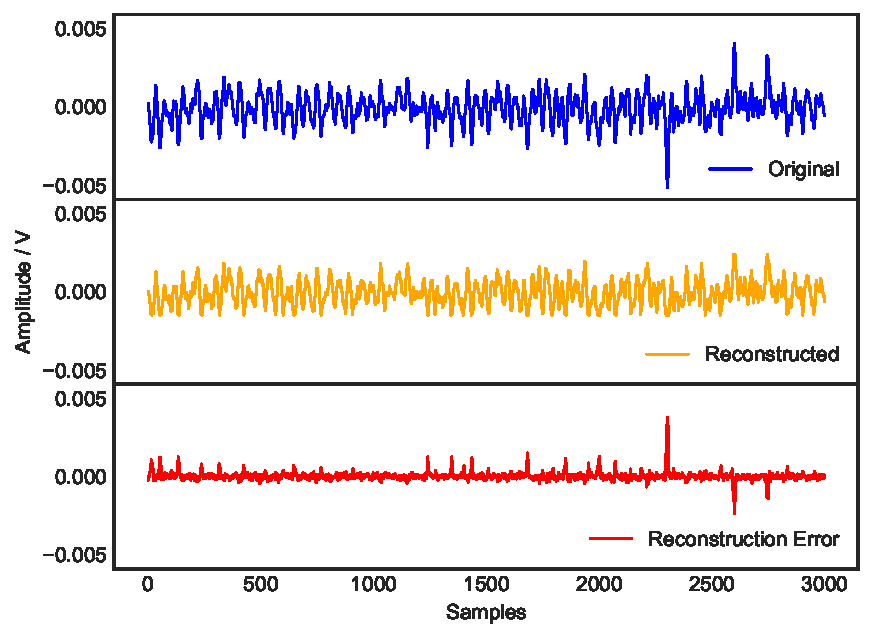
\includegraphics[width=1.0\textwidth]{fig/kmeans.pdf}
    \caption[K mean clustering plot]{Fancy figure goes here.}
    \label{fig:kmeanerror}
\end{figure}

Figure~\ref{fig:kmeanerror} shows an example of a reconstruction of testing data from synthetic segments created from a baseline signal of training data. The reconstruction error is the absolute difference between the reconstructed testing data and the actual testing data. Any spike in this reconstruction error, or a high average value over the entire length of the waveform, indicates that the motor is behaving differently from its optimum operation assumed from the baseline run.

\subsection{LSTM Recurrent Neural Networks}
\label{subsec:LSTM}

\subsubsection{Description of LSTM architecture}

%Machine learning is the science of programming computers in a manner that means they carry out tasks while not being explicitly programmed. In the past decade, machine learning has given us self-driving cars, practical speech recognition, effective web search, and a vastly improved understanding of the human genome.

Artificial neural networks (ANNs) are a biologically-inspired paradigm that provide a powerful set of techniques that provide solutions to many modern-day problems. In an age of rapidly increasing computational power from graphic processing units, ANNs are rapidly increasing in popularity.

ANNs are best described as a computing system made of many simplistic but highly interconnected layers, which process information by their dynamic state response to an external input. They are `connectionist machines' that simulate the densely interconnected cells that are found in a brain.

A form of ANN known as a recurrent neural network (RNN) consists of a structure of hundreds of thousands of units arranged in layers, which connect to other layers on either side. Some of these units are known as input units - with their role being to receive an information input that the network will attempt to learn about and process. Other types of unit on the other side of the network attempt to form a response to a learned input; these are known as output cells. In between the input and output units are hidden units, which make up the vast majority of the network. Similar to the manner in which neurons in a real brain operate, the links between separate units are assigned weights, in which a positive weight excites the connected unit, and a negative weight suppresses and inhibits the other unit.

RNNs operate by taking an input of information via the input units, triggering layers of hidden units before ending up at the output units. Each unit receives an input from the units that are located earlier in the network. These inputs are multiplied by the weights associated with the connections. The training process for a RNN typically involves the use of a feedback mechanism that propagates the network error backwards through the system.

%HOW THEY LEARN HOW THEY BACKPROPAGATE. WHAT MAKES A RECURRENT

Typical RNNs employ backpropagation training alongside stochastic gradient descent optimisation methods. The combination of these is known as a `backpropagation through time' algorithm. 

What this method involves is an input being passed forward through the neural network, layer by layer, until it reaches the output layer. The network's output is compared to the targeted output with the use of a loss function. An error value is then assigned to each of the `neurons' in the output layer. These error values are then passed backwards through the network, until each layer has an error associated with it that is proportional, and therefore representative of its contribution, to the original output \cite{Graves2012}. The effect of this process is to reduce the difference between the actual and intended output, by modifying the weights of the connections throughout the network. This means the network will be able to `figure something out' from an input, based on how the network has been trained beforehand.

However one problem with RNNs is that the error signal suffers from an exponential decay as it propagates through the network. This means that the front layers train very slowly, with the overall effect being that recurrent neural networks fail to learn in the presence of long lags in time between an input and target events. This problem was formalised by researchers and is known as the `vanishing gradient problem' \cite{hochreiter1991untersuchungen, hochreiter2001gradient}. By the mid-1990s the vanishing gradient problem had emerged as a major obstacle in the performance of recurrent neural networks.

LSTM (long short-term memory) is a type of RNN that was first proposed by \cite{Hochreiter:1997:LSM:1246443.1246450} as a way to overcome the vanishing gradient problem. An LSTM network is extremely well suited for learning tasks such as speech recognition \cite{Graves2005602}, handwriting recognition \cite{graves2008unconstrained} and music composition \cite{eck2002learning}. The properties of LSTM networks also make them extremely valuable for the prediction of time series \cite{gers2001applying}.

An LSTM consists of many recurrently connected subnets known as memory blocks. A memory block consists of three gates: the input, forget and output, as well as the cell state \cite{gers2000learning}. The core idea behind LSTMs is the cell state - which acts like a a conveyor belt. It lets information flow across the memory block unchanged, with the exception of a few minor linear interactions. These interactions are the gates - responsible for the removal or addition of information to the cell state.

%the optionally let memory through. each is is a sigmoid neural network and a multiplication operation the sigmoid function outputs a values between 0 and 1 which describes how much of each component should be let through we represent each of the following gates through the following equation.

\begin{figure}[t]
    \centering
    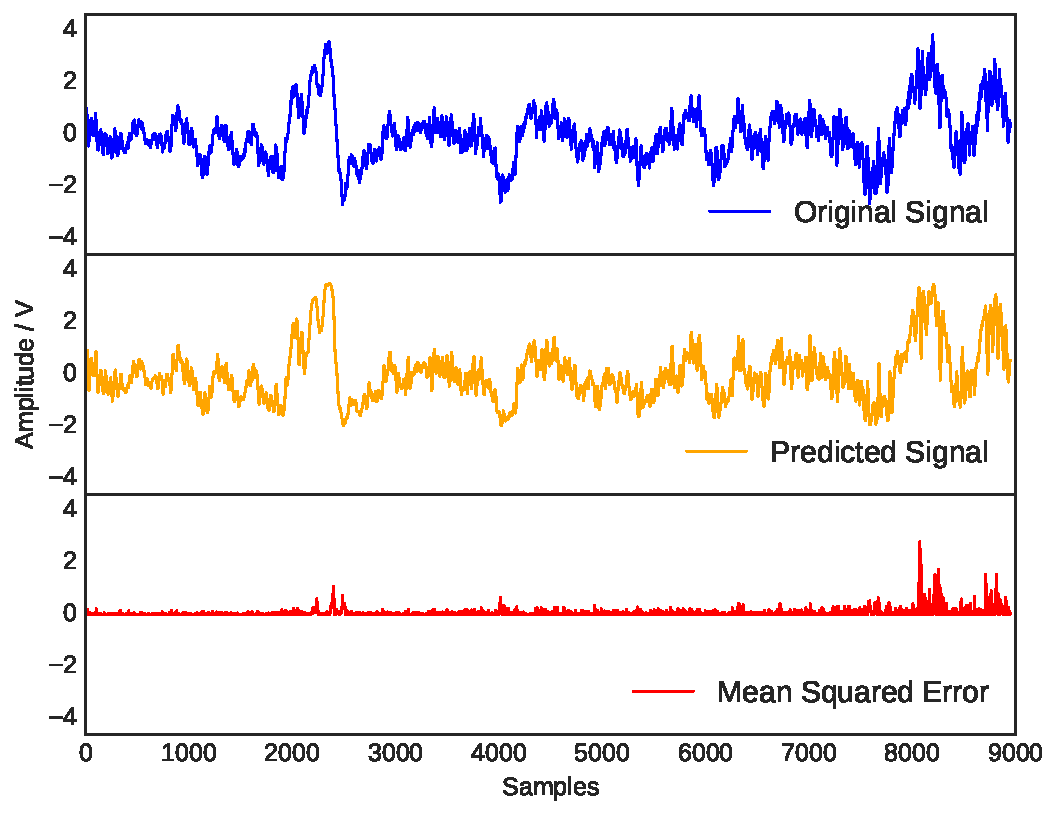
\includegraphics[width=1.0\textwidth]{neuralnetwork.pdf}
    \caption[Neural Network]{Using the LSTM functionality provided by \texttt{Keras}.}
    \label{fig:neuralnet}
\end{figure}

\begin{figure}[t]
    \centering
    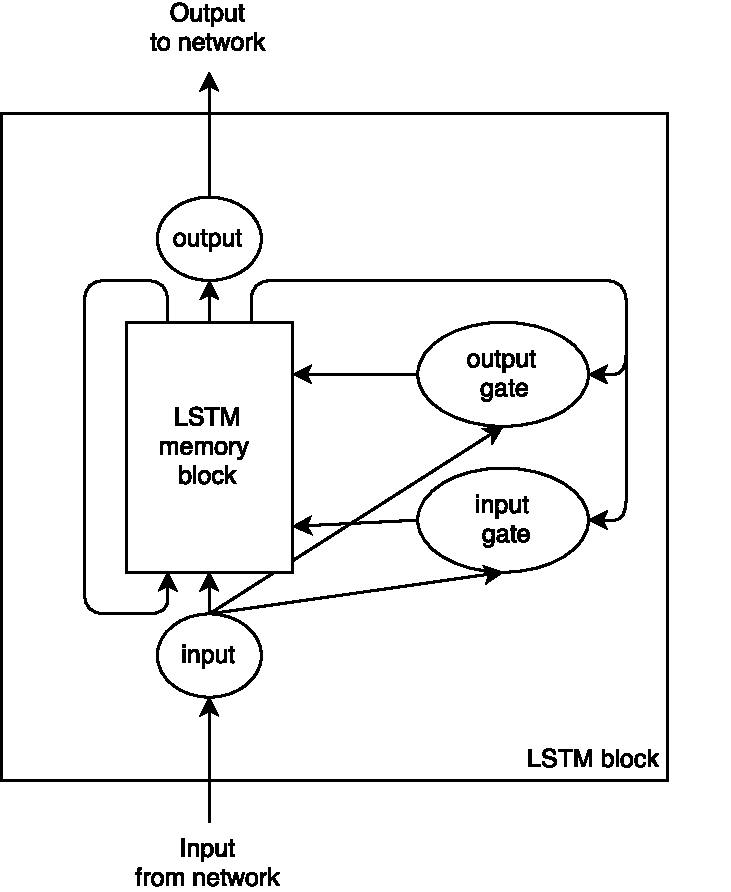
\includegraphics[width=0.5\textwidth]{LSTMcell.pdf}
    \caption[LSTM cell schematic]{Schematic of a long short-term memory block, used as a `neuron' in the hidden layers of a recurrent neural network.}
    \label{fig:lstmcell}
\end{figure}

A more mathematical description of the LSTM on how a layer of memory cells is updated begins with an input $x_t$ at timestep $t$. We define weight matrices as $W_i$,$W_f$,$W_c$,$W_o$,$U_i$,$U_f$,$U_c$,$U_o$ and bias vectors $b_i$,$b_f$,$b_c$,$b_o$.

At a time $t$, we define the input gate value $i_t$ and candidate value for the state of the memory cells $\widetilde{C}_t$ with,

\begin{equation}
    i_t = \sigma(W_i x_t + U_i h_{t-1} + b_i)~,
\end{equation}
\begin{equation}
    \widetilde{C}_t = \tanh(W_c x_t + U_c h_{t-1} + b_c)~.
\end{equation}

Next we calculate $f_t$, the value for the activation of the memory cells' forget gates,

\begin{equation}
    f_t = \sigma (W_f x_t + U_f h_{t-1} +b_f)~,
\end{equation}

where $\sigma$ is the activation function.

With these computed values we can then calculate $C_T$, the new state for the memory cells.

\begin{equation}
    C_t = i_t * \widetilde{C}_t + f_t * C_{t-1}~,
\end{equation}

And finally, one can now compute the value of the output gates and therefore outputs of the memory cells,

\begin{equation}
   o_t = \sigma(W_o x_t + U_o h_{t-1} + V_0 C_t + B_0)~,
   \label{output1}
\end{equation}
\begin{equation}
    h_t = o_t * \tanh(C_t)~.
\end{equation}

In the interest of more efficient computation, the LSTM model used in this report is a slight variant from what is most commonly described \cite{Graves2012}. The activation of a particular memory cell's output gate doesn't depend on the memory cell's state. This has the result of taking $V_0 = 0$ in Equation.~\eqref{output1}.

\subsubsection{LSTM implementation for anomaly detection}

%disadvantges
%ultimate 'black boxes'. Apart from defining the general archetecture of a network and perhaps initially seeding it with a random numbers, the user has no other role than to feed it input and watch it train and await the output. The final product of this activity is a trained network that provides no equations or coefficients defining a relationship (as in regression) beyond its own internal mathematics. The network 'IS' the final equation of the relationship.
%tend to be slower to train than other types of networks and sometimes require thousands of epochs. If run on a truly parallel computer system this issue is not really a problem an ANN can capture many kinds of relationships it allows the user to quickly and relatively easily model phenomena which otherwise may have been very difficult or imposible to explain otherwise.

\subsection{Rejected Methods of Anomaly Detection}
This subsection will include the methods considered for anomaly detection and why they were ultimately rejected to show that a wide range were considered but only certain few were used to ensure quality in the analysis.
